\documentclass{acm_proc_article-sp}

\begin{document}

\title{DataSeries: an efficient, flexible data format for structured serial data}
% Pretend we have one author, minimizes the space we waste on that.
\numberofauthors{1} 
\author{
\alignauthor
Eric Anderson, Martin Arlitt, Brad Morrey, Alistair Veitch  \\
 \affaddr{HP Labs. 1501 Page Mill Rd.  Palo Alto, CA} \\
 \email{\{eric.anderson4, martin.arlitt, brad.morrey, alistair.veitch\}@hp.com}
}

\maketitle
\begin{abstract}

DataSeries is an on-disk data format, run-time library, and set of
tools that is optimized for analyzing \textit{structured serial data},
which we define as an ordered series of records that share a common
structure.  This type of data commonly occurs as trace data in
computer systems, but since the format is essentially ordered RDBMS
tables, the need to maintain and analyze such data occurs in a large
number of scientific fields.

DataSeries has been optimized to be extremely space and CPU efficient,
while providing the flexibility to accommodate a very wide range of
record structures. We demonstrate the flexibility by describing the
many different types of data we have stored and analyzed in
DataSeries.  We examine the efficiency of DataSeries on a subset of
these types and demonstrate three improvements: 1) processing rates up
to two orders of magnitude better than existing formats; 2) ability to
store and analyze traces with hundreds of billions of records on
low-end servers; 3) compression ratios somewhat better than existing,
specialized formats when using the same generic compression algorithm,
and much better when compared to formats without built-in
compression. 

Finally, DataSeries software is open source, enabling others to take
advantage of these benefits.

\end{abstract}

% % A category with the (minimum) three required fields
% \category{H.4}{Information Systems Applications}{Miscellaneous}
% %A category including the fourth, optional field follows...
% \category{D.2.8}{Software Engineering}{Metrics}[complexity measures, performance measures]
 
% \terms{Structured serial data}

% \keywords{ACM proceedings, \LaTeX, text tagging} % NOT required for Proceedings

\section{Introduction}

Traces, recordings and measurements taken from computer systems,
networks and scientific infrastructure are vitally important for a
large variety of tasks. In every area of computer system design,
traces from existing systems have been used to validate hypotheses,
test assumptions and estimate performance. This is true of I/O
subsystems~\cite{IORef,Ji03,Uysal03}, processor
systems~\cite{ProcRef}, network systems~\cite{NetRef} and memory
systems~\cite{MemRef}, among others. Traces and logs are also
extremely useful for fault-finding, auditing and debugging purposes
~\cite{DebugRef}. Traces composed of failure data have been used to
determine system reliability~\cite{ReliabilityRef, Schroeder07,
Pinheiro07}. Trend analyses of performance information is a core
operation of various management tools~\cite{MgmtRef}. Specific to the
area of I/O and storage systems alone, we found that almost 60\% of
papers published in the File and Storage Technologies (FAST)
conferences have used traces of one sort or another.  Scientific and
medical instrumentation can also generate large amounts of
data~\cite{SciRef}, which also needs to be stored, filtered and
analyzed.

The data stored in each of these diverse uses is {\it structured
serial data}, which we define as a series of records, each record
having a specified structure (i.e., containing the same set of
variables). Structured serial data has four defining characteristics:
its structure is record-oriented; it is typically written only once,
not modified afterward, and is read many times; it is usually ordered
in some manner, e.g., chronologically; and it is typically read in a
sequential manner.  Traditionally, researchers and developers have
accomplished the tasks of collecting, storing, and analyzing this type
of data using formats, libraries and software which are customized to
the particular task at hand.  Unfortunately, such approaches
significantly limit both flexibility and reusability, and often
performance.  For instance, if a binary format is used, it may be
difficult to add new items of information or remove obsolete
information.  More flexible formats (e.g., text or XML) are not
amenable to efficient analysis or storage.  Traditional databases
generally store data without compression, requiring large amounts of
disk space for storage, and are typically not optimized for the
specific types of processing used on structured serial data.  One of
the key contributions of this work is the specific storage format and
optimizations that make it possible to very efficiently store and
analyze this type of data, without requiring excessive amounts of disk
storage or computational resources.

Another, often overlooked advantage of having a one-size-fits-all
trace format is the ease of use provided in data analysis. In our own
work, we have combined disparate trace types (block level I/O, process
accounting, system call, NFS, batch scheduler, and system performance
traces) in various combinations. Having a single software system and
trace format that can work with each of these trace types through
merge and analysis operations greatly facilitates the ease of
analysis. A related advantage is scientific; reproducibility is
enhanced and interpretation is simplified.  The authors have
experienced, both personally and anecdotally, the difficulty of
reproducing results with ``old'' trace files and software (often just
finding software and getting it to compile can be extremely
problematic). We observe that of the 101 papers published in the
history of FAST, 57 used traces in some way; the traces used in these
papers were of at least 45 different formats.  Several papers even
used 4-5 different types (e.g.,~\cite{arc03, ellard03}).

There are five key properties that are desired of a data format
and analysis system for structured serial data:

\begin{enumerate}

\item \textbf{Storage efficiency}: the data should be stored in as few
bytes as possible.

\item \textbf{Access efficiency}: accessing, interpreting and encoding
trace data, whether reading or writing, should make efficient use of
CPU and memory resources.

\item \textbf{Flexibility}: adding additional fields should not affect
users of the trace data.  Removing or modifying data fields should
only affect users who use those fields and the system should support
catching incorrect usage.  Further, the format should not constrain
the type of data being stored, and should allow multiple record types
in a single file.

\item \textbf{Self-describing}: the data set should contain the
metadata that describes the data.

\item \textbf{(Re)Usability}: the data format should have an associated
programming interface that is both expressive and easy to use.

\end{enumerate}

Although numerous tracing and measurement systems have been developed
over the last 20-30 years, we are not aware of any that meet all of
these requirements. We analyze some of these in our description of
related work (section~\ref{sec:related}).

We provide four primary contributions in this paper.  First, we
introduce DataSeries, a data format and associated library, which was
specifically designed to meet the five key properties discussed above.
Second, we discuss how DataSeries can support very large datasets
(e.g., hundreds of billions of records) on modest systems.  Third, we
describe how we have used DataSeries in practice to store a wide
variety of data types.  Fourth, we demonstrate the performance and
storage efficiency of DataSeries in a set of controlled experiments,
using empirical data sets. We show that the performance of DataSeries
exceeds the performance of common trace formats and databases by at
least a factor of two, and in some cases up to an order of
magnitude. DataSeries also requires far less disk space (factors vary
from 4X to 8X in test workloads).

Since DataSeries software is publicly available (under a BSD software
license), and given the benefits of DataSeries that we demonstrate, we
argue that DataSeries should be considered for use by any application
that needs to store large amounts of structured serial data. Indeed, a
storage industry group\footnote{name withheld for blinding purposes}
has chosen DataSeries as a standard format for I/O trace data, and is
currently specifying the semantics of the fields.

The remainder of this paper is organized as follows.
Section~\ref{sec:related} describes the strengths and weaknesses of
existing storage technologies relative to DataSeries.
Section~\ref{sec:design} describes the design of DataSeries, including
on-disk and in-memory formats.  Section~\ref{sec:programming}
describes the programming interface for DataSeries.
Section~\ref{sec:results} presents empirical and benchmark results
from our use of DataSeries to illustrate and quantify the benefits of
DataSeries.  Section~\ref{sec:discussion} describes our experiences
with using DataSeries, and Section~\ref{sec:conclusions} concludes the
paper with a summary of our work and a list of future directions.

\section{Related Work}\label{sec:related}

We classify the related work into three categories:
those that use a customized binary format, those that use a
text-based format, and relational database systems. 

Custom binary formats are usually serialized or directly written
versions of an in-memory data structure.  As such, they usually
achieve properties 1 and 2, and fail to achieve properties 3-5,
although as we will show in the results, unless the authors are
careful, they can also fail to achieve property 2.

Text base formats such as column separated value, or XML usually
achieve properties 3 and 4, and XML achieves property 5.  However,
they fail to achieve property 1, and can fail property two by multiple
orders of magnitude.  As we show in our results even very tuned CSV
implementations can only get to within 2-7$\times$ the
access-efficiency of DataSeries, and x-y$\times$ for the storage
efficiency.  {\bf TODO: need to re-do these experiments at least to
measure the file sizes, and potentially with Tfrac text files,
although I suspect people would use sec.usec in a block I/O trace}

Relational databases achieve properties 3, 4, and 5. RDBMS's were
designed to handle updates, so do very limited compression drastically
hurting their storage efficiency (property 1).  Our results show
$>$10x improvement on storage efficiency for DataSeries over
MySQL. {\bf TODO: check the exact sizes, should be around there.}
Similarly, the generality of SQL can hurt it.  Even for fairly simple
queries running entirely in the database, DataSeries runs 2-7$\times$
faster than MySQL. {\bf TODO: re-do these numbers with parallel
decompression, etc.}  Retrieving the data for a more complicated
calculation on the client would further slow the relative performance.

\section{Design}\label{sec:design}

DataSeries is intended to provide streaming access to structured serial
data. Corresponding
to the first four properties\footnote{The fifth property, an expressive
programming interface, is described in Section~\ref{sec:programming}.}
described in the introduction, DataSeries was designed with the
following goals in mind. First, it should be very storage
efficient. Second, it must be efficient to encode, decode and
interpret the data.  Third, the format should not constrain the
types of information to be stored. Fourth, the internal data must be
self-describing, i.e., the names and types of the data stored have to
be determined by the contents of the file itself, rather than 
externally.

DataSeries' data model is conceptually very similar to that used by
relational databases.  Logically, a DataSeries file is composed of an
ordered sequence of {\it records}, where each record is composed from
a set of {\it fields}. Each field has a {\it field-type} (e.g.,
integer, string, double, boolean) and a name. A DataSeries record is
analogous to a row in a conventional relational database. We call the
type of a row the {\it extent-type} because an {\it extent} contains a
collection of rows with the same fields and field-types.

A single DataSeries file comprises a collection of extents
(potentially with different extent-types), plus a header and
extent-type extent at the beginning of the file, and an index extent
and trailer at the end of the file. Figure~\ref{fig:dsorg} shows this
organization.  The extent-type and index extents are the same as the
other extents in the file except that their names and extent-types are
hard-coded in the library.

\begin{figure*}
% \vspace{-0.6cm}
\hfil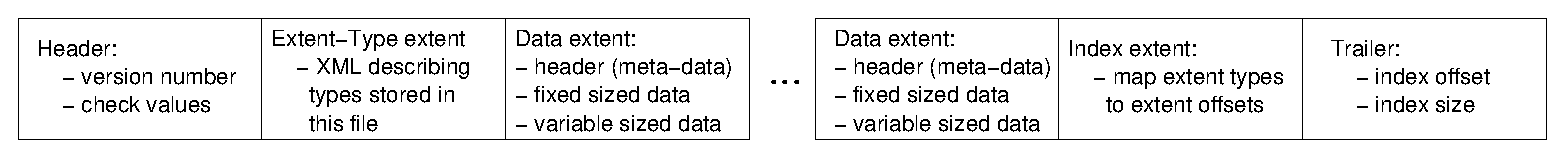
\includegraphics[width=6.5in]{tr-fig/ds-format2.eps}\hfil
\caption{Internal structure of a DataSeries file. }
\label{fig:dsorg}
% \vspace{-2mm}
\end{figure*}

The header on a DataSeries file contains the DataSeries file version,
and five check values to determine the encoding format for integers
and doubles.  DataSeries files are always written out using the native
formats of the system doing the writing. We did this to minimize
byte-swapping overheads, as usually the architecture reading the files
is the same as the architecture writing the files.  The library
transparently does endianness conversions in the rare circumstances
that this is not true, and also provides a ``repack'' utility for
explicit conversion.

Immediately following the header is the extent-type extent. Records in
this extent have a single string-valued field, each of which 
contains an XML specification that defines the extent-types of all the 
other extents in the file.  

When reading a DataSeries file, the trailer is read next.  It consists
of the offset and size (after compression) of the index extent.  The
offset is used to read the index extent, which has two fields, an
extent-type and an offset, to allow direct access to extents of a
single type.  The index and trailer are stored in this order, at the
end of the file, to enable efficient writing. The writer will often
not know, a priori, what the final extent sizes will be, so space for
the index cannot be allocated until after the extents have been
written.

The data extents themselves consist of a header, followed by the fixed
size data and the variable sized data.  Both fixed and variable sized
data may be compressed, using any one of a number of standard
compression algorithms~\cite{GZIP,BZIP,LZF,LZO}.  The header contains
metadata about the data in the extent, such as the compressed sizes of
the fixed and variable data, the number of records in the extent, the
uncompressed size of the variable length data, the compression mode,
the extent-type of the extent, and checksums of the extent before and
after compression to guard against hardware and software errors.
Checksum validation can be disabled during extent reading to improve
performance at the cost of reduced reliability.

Each row in the fixed size data is stored as a structure, with the
fields sorted by size and with padding between sizes.  In particular,
in each row, all of the boolean fields are packed, then all the byte
fields, padding is added to align to a 4 byte boundary, and then the 4
byte integer and variable offset pointers are packed.  Lastly, the
structure is padded to an 8 byte boundary and the 8 byte integer and
double fields are packed. When uncompressed, this layout allows for
very efficient access to data: every field can be accessed through a
pointer to the row, using a single addition and deference.  This
access method achieves goal two -- efficient decoding and
interpretation of the data.

DataSeries supports a number of options that control either the
interpretation of a field (e.g. can it be null), or the way the field
is represented prior to compression (\em{packed}, e.g. relative to
another field).  DataSeries also has some options for representation
of entire extents (e.g. ordering of the fields in a record).  The
packing options are handled transparently by DataSeries, the
interpretation options are checked against the field accessors.
Detailed explanation of the options can be found in the DataSeries
technical report~\cite{DSTechnicalReportSnapshot}.

\section{Programming}\label{sec:programming}

We introduce programming in DataSeries by means of a code sample,
which demonstrates how to read and process a DataSeries file.  

\subsection{Example analysis module}

The following example is extracted from the block I/O statistics
program used to perform the comparison with MySQL in
Section~\ref{sec:results}.  This is a very simple example that happens
to be equivalent to running {\tt dsstatgroupby Trace::BlockIO::HPUX
basic 'leave\_driver - enter\_driver' group by lvol\_number from
files...}

{ \footnotesize
\begin{verbatim}

// RowAnalysisModule handles the details of 
// getting each extent and iterating over the 
// rows using the ExtentSeries series.
class LatencyAnalysis : public RowAnalysis {
public:
    // The fields we will access in each row. 
    // In the real implementation, the field 
    // names are constructor arguments so that 
    // the module can operate on any fields of
    // the appropriate type.
    DoubleField start(series, "enter_driver");
    DoubleField end(series, "leave_driver");
    Int32Field group(series, "lvol_number");

    // Hash table for group-by operation
    typedef HashMap<int32, Stats *> mytableT;
    mytableT mystats;

    // This function is called for each row
    virtual void processRow() {
        // Stats class provides simple statistics
        // val method returns a field value
        Stats *stat = mystats[group.val()];
        if (stat == NULL) {
	    // make it easy to calculate 
	    // other stat types.
            stat = new Stats();
            mystats[group.val()] = stat;
        }
        stat->add(end.val() - start.val());
    }

    virtual void printResult() {
        cout << "lvol_num, mean, stddev\n";
        for_each(mytableT::iterator i, mystats) {
            cout << boost::format("%d, %.6g, %.6g\n") 
                % i->first % i->second->mean() 
                % i->second->stddev();
        }
    }
};

int main(int argc, char *argv[]) {
    // This defines the type of extents we want to 
    // process. We handle HPUX Block IO traces.
    TypeIndexModule source("Trace::BlockIO::HPUX");

    // Add in all the files to the source module.
    for(int i=1; i<argc; ++i) {
        source.addSource(argv[i]);
    }

    LatencyAnalysis analysis(source);

    // A real program would stack a whole 
    // collection of analysis in series.

    // Read all extents, delete after processing.
    analysis.getAndDelete();
    
    analysis.printResult();
    return 0;
}

\end{verbatim}
}

There are also lots of modules to help; see the TR.  Mention
dstypes2cxx here also.

\section{Performance Results}\label{sec:results}

...

\begin{table}
\centering
\begin{tabular}{|c|c|c|c|}\hline

               &            & ratio to & ratio to \\
    dataset    & size (MiB) & ds-base & be-bts-gz \\
\hline							   
ds-mcs-bts-tsr & 7648.98  & 1.133         & 1.077         \\
be-bts-gz      & 8239.15  & 1.052         & 1.000         \\
ds-base        & 8663.78  & 1.000         & 0.951         \\
\hline
\hline
\end{tabular}

\caption{Compression options for the data files sorted from the smallest 
to the largest.  Gzipped files can be stored little or big endian
(le/be) and small to big or big to small (stb/bts).  DataSeries files
can be stored with the fields padded only to the maximum column size
(mcs), with the fields stored big to small (bts), or with the time
field packed self relative (tsr). be-bts-gz is the original 1998 World
Cup trace format.}

\label{table:wc1998:compression}
\end{table}

\section{Discussion}\label{sec:discussion}

...

\section{Conclusions}\label{sec:conclusions}

...

DataSeries is open source that can be downloaded from {\tt
http://tesla.hpl.hp.com/opensource/}

\bibliographystyle{abbrv}
{\small
\bibliography{tr-references}
}
% You must have a proper ".bib" file
%  and remember to run:
% latex bibtex latex latex
% to resolve all references
%
% ACM needs 'a single self-contained file'!
%
\balancecolumns

\end{document}
